\section{Introduction}

  I have yet to see any problem, however complicated, which, when looked at in the right way did not become still more complicated.

  \begin{flushright}--- Poul Anderson\end{flushright}

  People working in the field of high energy physics have a tendency to concern themselves with attempting to solve problems that are incredibly complicated.
  So, perhaps, there is a touch of irony that the problem that they are trying to solve is not only incredibly fundamental, but also very simple to state.
  The question can be boiled down to -- what is the stuff in our universe made of?
  What immediately follows from this fundamental inquiry is how is matter made up of these things ; or to put it another way, how do the fundamental building blocks interact.

  In some sense particle physics tries to distill matter and the interactions therein down to the smallest possible level to which it can be broken down.
  Turns out that breaking these concepts down to this elementary level of specificity is an incredibly complicated process of which we have merely begun to scratch the surface.  As such,this paper focuses on a tiny fraction of these fundamental building blocks -- the elusive neutrino with the hope of just perhaps being able to untangle some of the myriad of secrets that it harbours.

  \subsection{The Standard Model}

Before the protagonist
\footnote{Really the ensemble cast, given that they come in three flavors, electron($e\nu$), muon ($\mu \nu$) and tau($\tau \nu$)and their respective antiparticles,}
of our story - the neutrino - can be formally introduced, the stage has to be set.
A good candidate to set the stage would be the standard model which describes three of the four known fundamental forces, electromagnetic, weak and strong interactions (it struggles to deal with  gravity) and classifying all known elementary particles \cite{Oerter}.
Just like any foundational theory that undergirds a sub-field of a subject, the standard model definitely wasn't developed in a day and as such, there is definite value in becoming familliar with the historical context surrounding the standard model in our quest to understand neutrinos.

One may definitely quibble about where our understanding of the fundamental particles starts from, after all, humans have been trying to find out the nature of our universe and the things that make it up going back as far as the 4th century BCE with Plato positing that everything is made up of 4 elements (water, wind, earth and fire)\cite{Timaeus}, but I think it makes sense to look at the elementary particles that make up the standard model as we know it today -- with the definite understanding that there may very well be physics that lies beyond the realm of the standard model.

At its core, the Standard Model consists of two main categories of particles: fermions, which make up matter, and bosons, which mediate interactions.
Fermions have $1/2$ integer spins while bosons have integer spins \cite{Oerter}.

\begin{figure}[H]
  % 
  \centering
  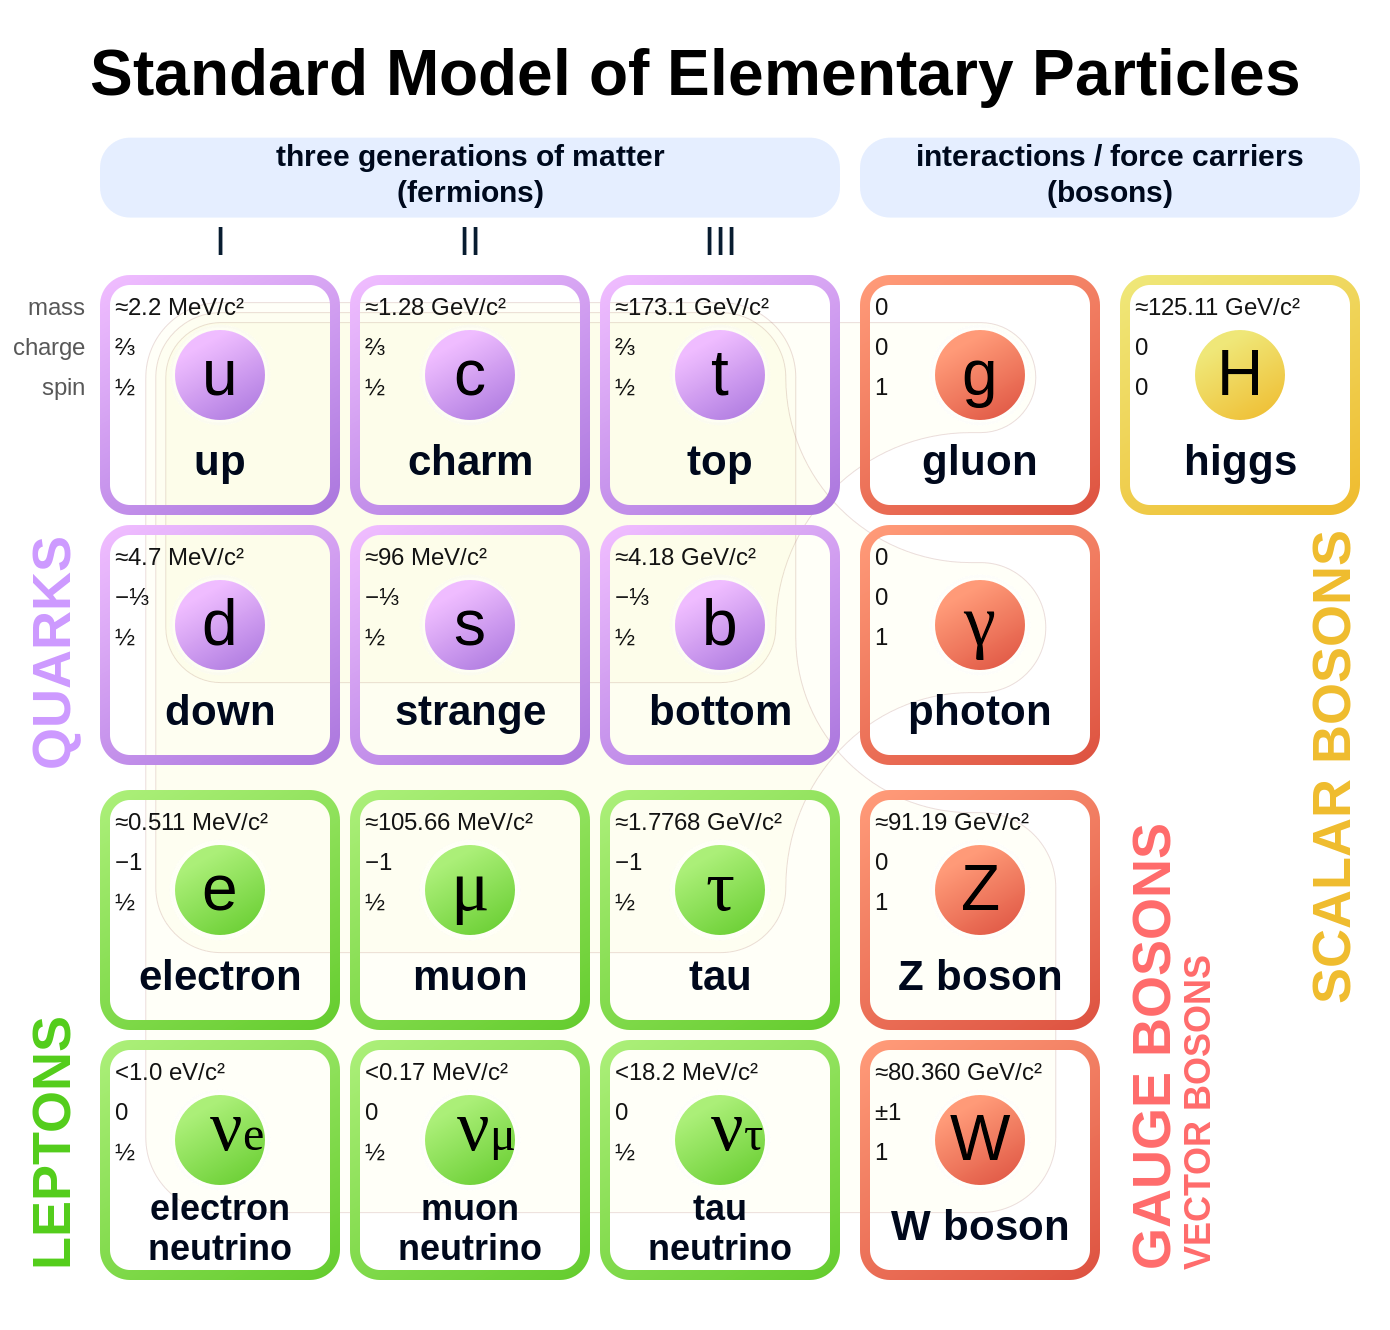
\includegraphics[width=80mm]{figures/sm.png}
  \caption{The Elementary Particles in the Standard Model \cite{standard_model}}
  \label{sm}
\end{figure}

The fermions can be further categorized into quarks and leptons.

\begin{figure}[H]
  % https://en.wikipedia.org/wiki/Quark#/media/File:Quark_structure_proton.svg
  \centering
  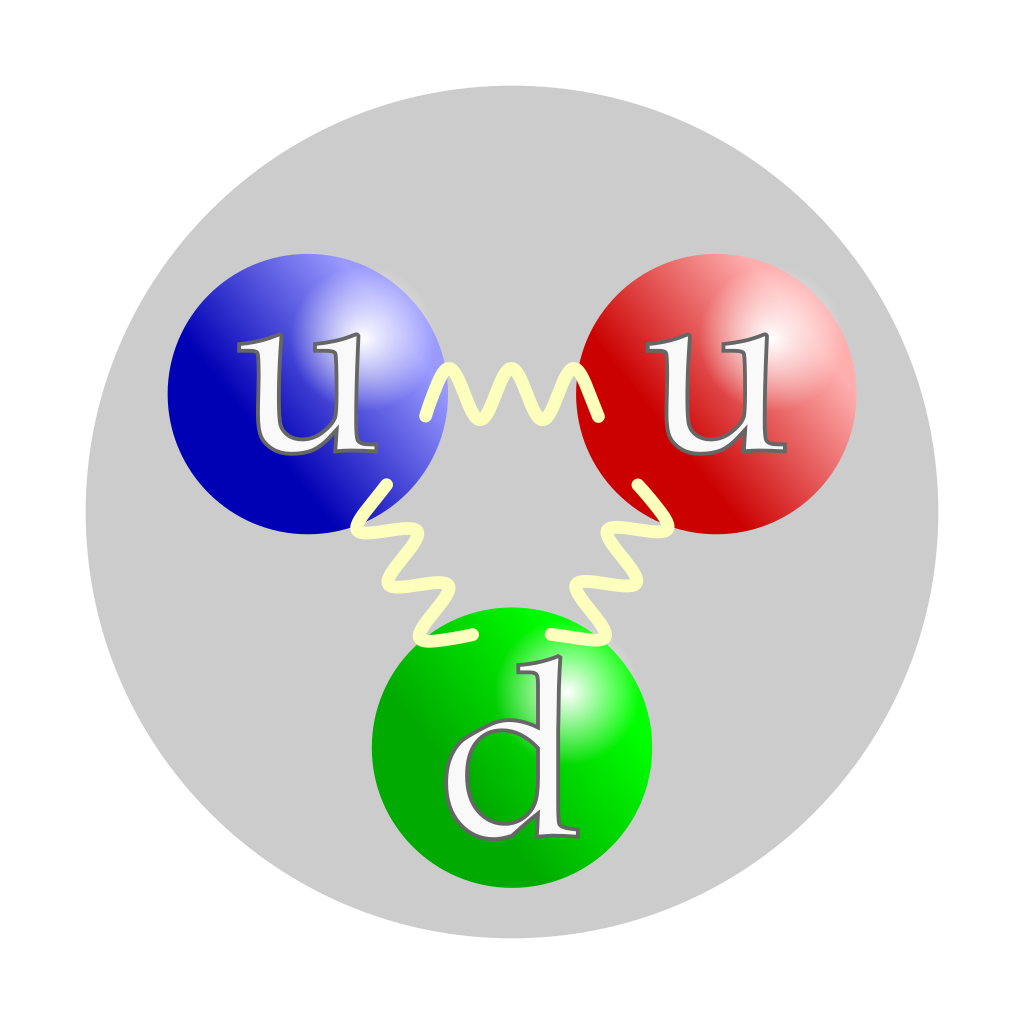
\includegraphics[width=100mm]{figures/protonQuarks.png}
  \caption{Quarks inside a proton.
    Labelled u for up and d for down\cite{quark}}
  \label{protonQuarks}
\end{figure}

Quarks are understood to be fundamental constituents of matter, forming the building blocks of protons, neutrons, and other hadrons (Composite subatomic particles that are made up of at least 2 quarks) \cite{quark_Brit_2024}.
Quarks interact with each other via the strong force.We have so far discovered 6 flavors of quarks -- up (\(u\)), down (\(d\)), charm (\(c\)), strange (\(s\)), top (\(t\)), and bottom (\(b\)).
Each flavor has different mass.
These masses and their interactions with other particles are crucial for the stability and properties of atomic nuclei \cite{Nave_quark}.

\begin{table}[h!]

  \centering
  \begin{tabular}{lrr}
    \toprule
    Quark Flavor & Approximate Mass (MeV/c\(^2\)) & Charge (e) \\
    \midrule
    Up (u)      & 2.2 - 3.0        & +\(\frac{2}{3}\) \\
    Down (d)    & 4.7 - 5.0        & -\(\frac{1}{3}\) \\
    Strange (s) & 95 - 105         & -\(\frac{1}{3}\) \\
    Charm (c)   & 1270 - 1720      & +\(\frac{2}{3}\) \\
    Bottom (b)  & 4180 - 4380      & -\(\frac{1}{3}\) \\
    Top (t)     & 172000 - 173000  & +\(\frac{2}{3}\) \\
    \bottomrule
  \end{tabular}
  \caption{Quark Flavors, Their Approximate Masses and Charges \cite{Nave_quark}}
  \label{quarkMass}
\end{table}

Each type of fermion carries a specific flavor and generation.
For instance, the electron ($e$) belongs to the first generation, while the muon ($\mu$) and tau ($\tau$) belong to the second and third generations, respectively \cite{Nave_lepton} \footnote{The neutrino, despite being elusive, plays a significant role in weak interactions and lepton family conservation.}.

The interactions between these particles are mediated by gauge bosons, which are the force carriers \cite{Gribbin_2000}\cite{Clark_2004}.
The Standard Model includes the following gauge bosons:

\begin{align}
 & \quad \text{Photon } (\gamma) \quad \text{(mediates electromagnetic force)} \\
                    & \quad \text{W and Z bosons } (W^\pm, Z^0) \quad \text{(mediates weak force)} \\
                    & \quad \text{Gluons } (g) \quad \text{(mediates strong force) \cite{Veltman_2004}}
\end{align}

The mathematical framework underpinning the Standard Model is primarily based on gauge theory, specifically the group $SU(3) \times SU(2) \times U(1)$.
Each of these groups corresponds to a different force:

\begin{align}
\text{Strong Interaction:} & \quad SU(3) \quad \text{(color charge)} \\
\text{Weak Interaction:} & \quad SU(2) \quad \text{(isospin)} \\
\text{Electromagnetic Interaction:} & \quad U(1) \quad \text{(hypercharge)}
\end{align}

The Higgs mechanism, a crucial part of the Standard Model, provides a mass to the W and Z bosons via spontaneous symmetry breaking.
The Higgs field $\phi$ can be parameterized as:

\begin{align}
\phi &= \frac{v+h}{\sqrt{2}}e^i{\frac{\chi}{v}}
\end{align}

where $h$, the Higgs boson and $\chi$, the Goldstone boson are real scalar fields which have no vacuum expectation value.
The mass terms for the gauge bosons arise when the Higgs field acquires a vacuum expectation value\cite{Bernardi_2008}.



  \subsection{Electroweak Interactions}